\documentclass[a4paper, 12pt]{article}

\newcommand\tab[1][.6cm]{\hspace*{#1}}
\usepackage[portuges]{babel}
\usepackage[utf8]{inputenc}
\usepackage{amsmath}
\usepackage{indentfirst}
\usepackage{graphicx}
\usepackage{multicol,lipsum}
\usepackage{blindtext}
\usepackage{verbatim}
\usepackage{textcomp}
\usepackage{hyperref}
\usepackage{float}
\usepackage{url}

\begin{document}
%\maketitle

\begin{titlepage}
	\begin{center}
	
	\begin{figure}[ht]
    \centering
    
\includegraphics[width=.44\textwidth]{Images/LogoUFSJ.PNG}
    \label{fig:Capturar.PNG}
    \end{figure}

    	\Huge{Universidade Federal São João del Rei}\\
		\Large{Curso de Ciência da Computação}\\ 

        \vspace{110pt}
        \textbf{\LARGE{
        \\
        \\
        \\
        Trabalho Prático 2: Documentação\\
        \vspace{0.5cm}
        \Large{Redes de Computadores I}
        \\
        \\
        \\
        }}
        
		\title{{\large{Título}}}
		\vspace{2.5cm}
	\end{center}
	    
    \begin{flushleft}
		\begin{tabbing}
		\\
		\\
		\\	
		\large{Discente: Julio Cesar da Silva Rodrigues}\\
	    \\
		\large{Docente: Rafael Sachetto Oliveira}\\
	    \end{tabbing}
    \end{flushleft}
	\vspace{1cm}
	
	\begin{center}
		\vspace{\fill}
			Novembro\\
		    2022
	\end{center}
\end{titlepage}

\tableofcontents
\newpage
\section{Introdução}

Como especificado no enunciado do trabalho prático proposto, serão apresentados de forma sumarizada, alguns aspectos abordados no desenvolvimento desta tarefa. Veremos as etapas envolvidas, soluções, obstáculos encontrados, entre outras observações, cujo objetivo eram estimular um melhor entendimento de programação de protocolos da camada aplicação e de transporte de forma prática. Para isto, é necessário novamente realizar a comunicação entre processos pela rede, utilizando informações como endereço de \emph{IP}, nome de domínio, número de porta, hospedeiro, entre outras.

Diante desta introdução, a tentativa foi de implementar tais protocolos da camada de aplicação e transporte adaptados para um servidor \emph{web}, ou seja, implementar um programa que seja capaz de lidar com um conjunto pequeno das mensagens que possuem o formato \emph{HTTP}, enviadas como requisições pelos clientes. E como pressuposto, o programa também deve ser capaz de formular as respostas adequadas no mesmo formato para formar o par de comunicação completo entre cliente e servidor. 

\section{Estrutura Geral}

Toda a concepção das estruturas de requisições e respostas, assim como as funções que às manipulam foram implementadas em linguagem C (excetuando a análise de resultados gráfica, que foi gerada utilizando a linguagem \emph{Python}). A implementação foi desenvolvida com o auxílio da ferramenta de controle de versionamento GitHub, e encontra-se disponível publicamente no repositório \url{https://github.com/juliorodrigues07/web_server_c}.

A organização do código se apresenta de forma bastante simples. Existe apenas um diretório fonte que corresponde basicamente à todas as operações executadas pelos servidor. Neste diretório, existem apenas os \emph{scripts} responsáveis pelo funcionamento dos servidores como um todo (.c e .h), e o principal que apenas direciona ao tipo de servidor desejado pelo usuário na utilização.

\pagebreak

\section{Estruturas de Dados e Funções}

No \emph{script server.h} (\emph{header} do servidor), encontram-se as estruturas de dados que definem cada requisição e cada resposta, e estas contém as seguintes variáveis:

\begin{itemize}
    \item \emph{request}
    \begin{itemize}
        \item \emph{bytes\_read}: Inteiro responsável por armazenar a quantidade de \emph{bytes} lidos de uma requisição qualquer;
        \item \emph{header}: \emph{String} que armazena o conteúdo da mensagem de requisição em si.
    \end{itemize}
    \item \emph{response}
    \begin{itemize}
        \item \emph{response\_buffer}: \emph{String} responsável por armazenar o conteúdo da mensagem de resposta;
        \item \emph{message\_length}: Inteiro responsável por armazenar o tamanho da mensagem de resposta;
        \item \emph{status}: Inteiro responsável por armazenar o estado da mensagem de resposta (200, 404, ...).
    \end{itemize}
\end{itemize}

Também são definidas algumas constantes importantes como número da porta, quantidade máxima de conexões, tamanho de cabeçalho, caminho e buffer, além claro de variáveis para controle das \emph{threads}.

\subsection{Função \emph{socket\_creation}}

Esta função, baseada fortemente no código de apoio disponibilizado junto ao enunciado deste trabalho prático (\emph{server\_tcp.c}), é responsável apenas por configurar a preparação da conexão (\emph{Opening, Binding, Listening...}) para a comunicação via \emph{socket TCP} do servidor com processos de outras máquinas, ou neste caso, com processos da máquina local.

\subsection{Função \emph{read\_header}}

O propósito desta função é bastante simples, esta apenas realiza a leitura da mensagem de requisição \emph{HTTP} enviada pelo cliente.

\subsection{Função \emph{client\_response}}

Nesta função, ocorrem o envio das respostas às requisições dos usuários. Atuando em conjunto com a função \emph{read\_header} mencionada anteriormente, esta primeiramente obtém a mensagem \emph{HTTP} de requisição, para então submetê-la ao "analisador" de mensagens \emph{HTTP} (\emph{parser}). Após realizada esta análise, o servidor envia a resposta correspondente na conexão \emph{socket TCP} existente entre o par. 

\subsection{Função \emph{http\_parser}}

Esta função tem como principal funcionalidade executar a análise das mensagens \emph{HTTP} de requisição que são enviadas pelos usuários. Por esta implementação apenas lidar com o método \emph{GET}, a primeira verificação feita é se este esta presente na linha de requisição da mensagem. Caso não estiver, é enviada ao usuário um código indicando que a requisição enviada está mal formulada (400 - \emph{Bad Request}).

Em casos mais gerais, esta função, com o auxílio de uma segunda que será explanada na próxima seção, fará a interpretação da mensagem de requisição \emph{HTTP} recebida, para então direcionar as solicitações desejadas como arquivos, ou informar outros códigos de erro presentes na especificação do protocolo de mensagens.

\subsection{Função \emph{laod\_file}}

Esta função será a responsável por retornar as mensagens de erro ou os arquivos desejados, conforme o conteúdo especificado na linha de requisição da mensagem \emph{HTTP} pelo usuário.

\subsection{Função \emph{iterative\_server}}

O tipo de servidor mais simples presente na implementação, este atende a requisição de apenas um cliente por vez (única conexão) de forma bloqueante, ou seja, um vez realizada a conexão, o servidor deverá aguardar indefinidamente até que o usuário envie-o uma mensagem de requisição \emph{HTTP};

\subsection{Função \emph{fork\_server}}

O modo de operação que apresentou maiores problemas, o servidor utilizando \emph{fork} se mostrou bastante ineficiente devido à falta de ajuste no controle de quantos processos são criados ao longo do tempo à medida que chegam mensagens de requisição. A partir do momento que é realizada a conexão, é criado um processo filho para responder à tal, mas há grandes deficiências na implementação deste tipo de servidor que serão discutidas mais adiante.

\subsection{Funções \emph{thread\_server} e \emph{consumer}}

Talvez o tipo de servidor que apresentou o maior desafio na implementação, este modo de operação também possui defeitos, mas aparentemente não tão graves quanto o servidor baseado em \emph{fork}. Aqui, um número fixo de \emph{threads} é criado, utilizando como parâmetro uma constante definida no \emph{header}. Após a criação das \emph{threads}, uma fila de tarefas também de tamanho fixo é mantida, para serem alocadas às \emph{threads} de acordo com disponibilidade para consumir as requisições.

\subsection{Função \emph{concurrent\_server}}

Surpreendentemente o tipo de servidor que não apresentou tantos obstáculos na implementação, este se difere em relação ao modo mais básico, apenas na sua forma de operação não bloqueante (não totalmente). Este tipo de servidor suporta várias conexões simultâneas, mas somente irá bloquear para responder as mensagens de requisição \emph{HTTP}, quando de fato houverem dados a serem processados enviados por um cliente.

\section{Análise de Resultados}

Nesta seção, discutiremos algumas métricas obtidas utilizando a ferramenta \emph{Siege}, na execução de testes com os diferentes servidores presentes na implementação.

É importante citar que os testes foram realizados mantendo o tempo fixo (dez segundos) em todos os modos de servidores e com quaisquer números de clientes simultâneos. Foram também utilizados parâmetros padrão da ferramenta, ou seja, o número máximo de usuários concorrendo é limitado à 255, e não foi atribuído nenhum intervalo específico o qual os usuários deveriam respeitar entre o envio das requisições. 

Por fim, os testes foram executados sempre utilizando o mesmo arquivo como parâmetro (\emph{cat.jpg}) na requisição, e também foram executados cinco vezes com cada número de clientes em cada modo de servidor, para então calcular a média e exibir as informações aproximadas. O gráfico relacionando o número de requisições respondidas por segundo, com a quantidade de usuários concorrente em cada modo de servidor é exibido na Figura \ref{fig:exampleFig1}.

\begin{figure}[H]
    \centering
    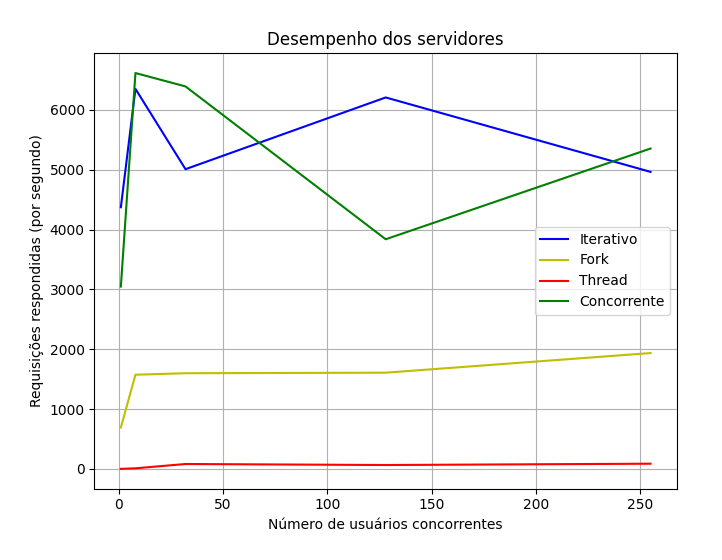
\includegraphics[width=0.98\textwidth]{Images/graph.png}
    \caption{Gráfico comparativo do desempenho dos servidores}
    \label{fig:exampleFig1}
\end{figure}

Podemos observar nitidamente no gráfico, que os dois tipos de servidores que presumidamente deveriam ser os que obteriam o melhor desempenho, apresentaram níveis bem abaixo da expectativa em relação aos seus concorrentes mais simples. Esperamos discutir melhor essa disparidade na próxima seção, apontando possíveis falhas que levaram ao desempenho muito abaixo do esperado pelos servidores \emph{fork} e \emph{thread}.

O resumo exibindo as médias dos valores brutos obtidos a partir dos testes de dez segundos são sumarizados na Tabela \ref{tab:exampleTab1}:

\begin{table}[H]
    \centering
    \caption{Número de requisições respondidas por cada servidor (10 segundos)}\vspace{0.3cm}
    \label{tab:exampleTab1}
    \begin{tabular}{c|c|c|c|c}
     \textbf{Usuários} & \textbf{Iterativo} & \textbf{Fork} & \textbf{Thread} & \textbf{Concorrente}\\
     1 & 43728 & 6912 & 10 & 30468\\
     8 & 63511 & 15743 & 96 & 66165\\
     32 & 50090 & 15992 & 822 & 63921\\
     128 & 62085 & 16085 & 646 & 38386\\
     255 & 49643 & 19361 & 874 & 53546
    \end{tabular}
\end{table}

\section{Limitações}

A principal falha encontrada até o momento na implementação atual, se encontra no servidor que utiliza \emph{forks}. Esperar o término do processo filho não seria uma opção, já que isto faria basicamente com que seu funcionamento seguisse o princípio do servidor iterativo. O tempo de espera inserido (\emph{timeout}) também não se mostra adequado, já que aparentemente vários processos "zumbis" são criados, acarretando em aumento demasiado no processamento e no nível de ocupação da memória principal (\emph{memory leak}), à medida que são ampliados os parâmetros como tempo e número de clientes concorrentes.

A segunda falha está no servidor que utiliza \emph{threads}. O tempo de ociosidade escolhido também não se mostra adequado, mantendo o servidor a maior parte do tempo omisso à resposta das requisições. Assim como o servidor \emph{fork}, deve-se encontrar o equílibrio nos parâmetros com testes intensivos para evitar a criação de \emph{forks} ou \emph{threads} em excesso ou de forma escassa.

\section{Compilação e Execução}

Antes de discutir quaisquer detalhes de compilação e execução, é importante citar que a execução dos vários tipos de servidor pode requerer uma mudança no número da porta para possibilitar a abertura da conexão no \emph{socket TCP}. Esta alteração deve ser feita diretamente no código (\emph{server.h}) onde está definida a constante do número de porta (\emph{PORT\_NUMBER}).\\

\noindent Para compilar o programa, basta executar o seguinte comando via terminal:

\begin{center}
    \boxed{\textbf{\large{make}}}
\end{center}

\noindent Na execução, basta executar o comando no seguinte modelo via terminal:

\begin{center}
    \boxed{\textbf{\large{make }} $$<\textit{nome do servidor}>$$}
\end{center}

\noindent $<\textit{nome do servidor}>$ \(\rightarrow\) [iterative, fork, thread ou concurrent]\\

\noindent Para testar utilizando o \emph{software Siege}, basta digitar o comando no seguinte modelo em outra aba de terminal:

\begin{center}
    \boxed{\textbf{\large{siege -twS -cx http://localhost:y/z}}}
\end{center}

\pagebreak

\noindent Em que:
\begin{itemize}
    \item \(w\): Tempo em segundos;
    \item \(x\): Quantidade de usuários simultâneos;
    \item \(y\): Número da porta;
    \item \(z\): Nome ou caminho do arquivo.
\end{itemize}

\noindent Segue um exemplo: 

\begin{center}
    \boxed{\textbf{\large{siege -t10S -c128 http://localhost:2000/cat.jpg}}}
\end{center}

\noindent Também pode-se testar individualmente pelo navegador, executando a seguinte pesquisa exemplo: 

\begin{center}
    \boxed{\textbf{\large{http://127.0.0.1:2000/index.html}}}
\end{center}

\noindent Por fim, os arquivos presentes no diretório \emph{files} são exibidos na Tabela \ref{tab:exampleTab2}:
\begin{table}[H]
    \centering
    \caption{Arquivos presentes no diretótio \emph{files}}\vspace{0.3cm}
    \label{tab:exampleTab2}
    \begin{tabular}{c|c|c}
     400.html & 404.html & 413.html\\
     index.html & ca.jpg & f1.gif\\
     & batman.mp4 &
    \end{tabular}
\end{table}

\section{Considerações Finais}

Neste trabalho, foi construído parte da comunicação entre um par (\emph{Cliente-Servidor}) para o envio de requisições e respostas no formato de mensagem \emph{HTTP} em rede. Portanto, o objetivo principal era tentar compreender de forma mais clara, como ocorrem os processos de comunicação e transmissão de dados na camada de aplicação e de transporte. 

Pela manipulação de estruturas como \emph{threads} não ter se mostrado trivial, considero que a implementação do servidor com fila de tarefas e \emph{threads} ofereceu o maior desafio, juntamente à utilização da ferramenta \emph{Siege} na tentativa de obter boas métricas para demonstrar o comportamento de cada tipo de servidor e seu desempenho bruto.

Com este exemplo didático, podemos observar de forma nítida, a complexidade por trás da transmissão de dados, mesmo que em volume pequeno, que podem ser requisitados de forma constante em quaisquer redes de computadores, sejam estas locais, regionais, ou globais como a \emph{internet}. 

\section*{Referências}

\begin{itemize}
    \item Speed testing your website performance with Siege: Part One: \url{https://www.euperia.com/wrote/speed-testing-your-website-with-siege-part-one};
    \item Series of posts on HTTP status codes: \url{https://evertpot.com/http/};
    \item Load Testing Web Servers with Siege Benchmarking Tool: \url{https://www.tecmint.com/load-testing-web-servers-with-siege-benchmarking-tool/};
    \item How to install Siege on Ubuntu: \url{https://linuxhint.com/install-siege-ubuntu/};
    \item Material disponível no portal didático na disciplina de Redes de Computadores I.
\end{itemize}

\end{document}
